\documentclass{article}\usepackage[]{graphicx}\usepackage[]{color}
%% maxwidth is the original width if it is less than linewidth
%% otherwise use linewidth (to make sure the graphics do not exceed the margin)
\makeatletter
\def\maxwidth{ %
  \ifdim\Gin@nat@width>\linewidth
    \linewidth
  \else
    \Gin@nat@width
  \fi
}
\makeatother

\definecolor{fgcolor}{rgb}{0.345, 0.345, 0.345}
\newcommand{\hlnum}[1]{\textcolor[rgb]{0.686,0.059,0.569}{#1}}%
\newcommand{\hlstr}[1]{\textcolor[rgb]{0.192,0.494,0.8}{#1}}%
\newcommand{\hlcom}[1]{\textcolor[rgb]{0.678,0.584,0.686}{\textit{#1}}}%
\newcommand{\hlopt}[1]{\textcolor[rgb]{0,0,0}{#1}}%
\newcommand{\hlstd}[1]{\textcolor[rgb]{0.345,0.345,0.345}{#1}}%
\newcommand{\hlkwa}[1]{\textcolor[rgb]{0.161,0.373,0.58}{\textbf{#1}}}%
\newcommand{\hlkwb}[1]{\textcolor[rgb]{0.69,0.353,0.396}{#1}}%
\newcommand{\hlkwc}[1]{\textcolor[rgb]{0.333,0.667,0.333}{#1}}%
\newcommand{\hlkwd}[1]{\textcolor[rgb]{0.737,0.353,0.396}{\textbf{#1}}}%

\usepackage{framed}
\makeatletter
\newenvironment{kframe}{%
 \def\at@end@of@kframe{}%
 \ifinner\ifhmode%
  \def\at@end@of@kframe{\end{minipage}}%
  \begin{minipage}{\columnwidth}%
 \fi\fi%
 \def\FrameCommand##1{\hskip\@totalleftmargin \hskip-\fboxsep
 \colorbox{shadecolor}{##1}\hskip-\fboxsep
     % There is no \\@totalrightmargin, so:
     \hskip-\linewidth \hskip-\@totalleftmargin \hskip\columnwidth}%
 \MakeFramed {\advance\hsize-\width
   \@totalleftmargin\z@ \linewidth\hsize
   \@setminipage}}%
 {\par\unskip\endMakeFramed%
 \at@end@of@kframe}
\makeatother

\definecolor{shadecolor}{rgb}{.97, .97, .97}
\definecolor{messagecolor}{rgb}{0, 0, 0}
\definecolor{warningcolor}{rgb}{1, 0, 1}
\definecolor{errorcolor}{rgb}{1, 0, 0}
\newenvironment{knitrout}{}{} % an empty environment to be redefined in TeX

\usepackage{alltt}

\usepackage{amsmath, amssymb}
\usepackage{graphicx}
\usepackage{hyperref}
\IfFileExists{upquote.sty}{\usepackage{upquote}}{}
\begin{document}

\title{Pol Sci 630: Problem Set 4 - Regression Model Estimation}

\author{Prepared by: Anh Le (\href{mailto:anh.le@duke.edu}{anh.le@duke.edu})}

\date{Due Date: Tuesday, September 22nd, 2015, 10 AM (Beginning of Class)}

\maketitle

Note 1: It is absolutely essential that you show all your work, including intermediary steps, and comment on your R code to earn full credit.

Note 2: Please use a *single* PDF file created through knitr to submit your answers. knitr allows you to combine R code and \LaTeX \ code in one document, meaning that you can include both the answers to R programming and math problems. Also submit the source code that generates the PDF file (i.e. .Rnw file)

Note 3: Make sure that the PDF files you submit do not include any references to your identity. The grading will happen anonymously. You can submit your answer at the following website: \url{http://ps630-f15.herokuapp.com/}

\section*{1. Create a data frame (4 points)}

\subsection*{a)}
First, \verb`set.seed(2)`. Then, create a data frame with 1000 rows and 3 variables as follows:
\begin{enumerate}
\item \verb`var_norm`: a normal variable with mean = 5, sd = 10
\item \verb`var_binom`: a binomial variable with number of trial = 10, probability of success = 0.5
\item \verb`var_poisson`: a Poisson variable with $\lambda = 4$
\end{enumerate}

(Recall how to generate random sample from various distributions from previous labs.)

\subsection*{b)}

Plot the histograms of the three variables, arranging them nicely (with \verb`fig.width()`, \verb`fig.height()`, \verb`par(mfrow)` as you see fit). Brownie point if you plot using a for loop instead of writing \verb`hist` three times.

\textbf{Solution}

\begin{knitrout}
\definecolor{shadecolor}{rgb}{0.969, 0.969, 0.969}\color{fgcolor}\begin{kframe}
\begin{alltt}
\hlcom{# Create the data frame}
\hlkwd{set.seed}\hlstd{(}\hlnum{2}\hlstd{)}
\hlstd{my_dataframe} \hlkwb{<-} \hlkwd{data.frame}\hlstd{(}\hlkwc{var_norm} \hlstd{=} \hlkwd{rnorm}\hlstd{(}\hlnum{1000}\hlstd{,} \hlkwc{mean} \hlstd{=} \hlnum{5}\hlstd{,} \hlkwc{sd} \hlstd{=} \hlnum{10}\hlstd{),}
                           \hlkwc{var_binom} \hlstd{=} \hlkwd{rbinom}\hlstd{(}\hlnum{1000}\hlstd{,} \hlkwc{n} \hlstd{=} \hlnum{10}\hlstd{,} \hlkwc{prob} \hlstd{=} \hlnum{0.5}\hlstd{),}
                           \hlkwc{var_poisson} \hlstd{=} \hlkwd{rpois}\hlstd{(}\hlnum{1000}\hlstd{,} \hlkwc{lambda} \hlstd{=} \hlnum{4}\hlstd{))}
\end{alltt}
\end{kframe}
\end{knitrout}

\begin{knitrout}
\definecolor{shadecolor}{rgb}{0.969, 0.969, 0.969}\color{fgcolor}\begin{kframe}
\begin{alltt}
\hlcom{# Plot the histogram (nicely)}
\hlkwd{par}\hlstd{(}\hlkwc{mfrow} \hlstd{=} \hlkwd{c}\hlstd{(}\hlnum{1}\hlstd{,} \hlnum{3}\hlstd{))}
\hlkwa{for} \hlstd{(i} \hlkwa{in} \hlnum{1}\hlopt{:}\hlnum{3}\hlstd{) \{}
  \hlkwd{hist}\hlstd{(my_dataframe[ , i],}
       \hlkwc{xlab} \hlstd{=} \hlkwd{colnames}\hlstd{(my_dataframe)[i],} \hlkwc{main} \hlstd{=} \hlkwa{NULL}\hlstd{)}
\hlstd{\}}
\end{alltt}
\end{kframe}
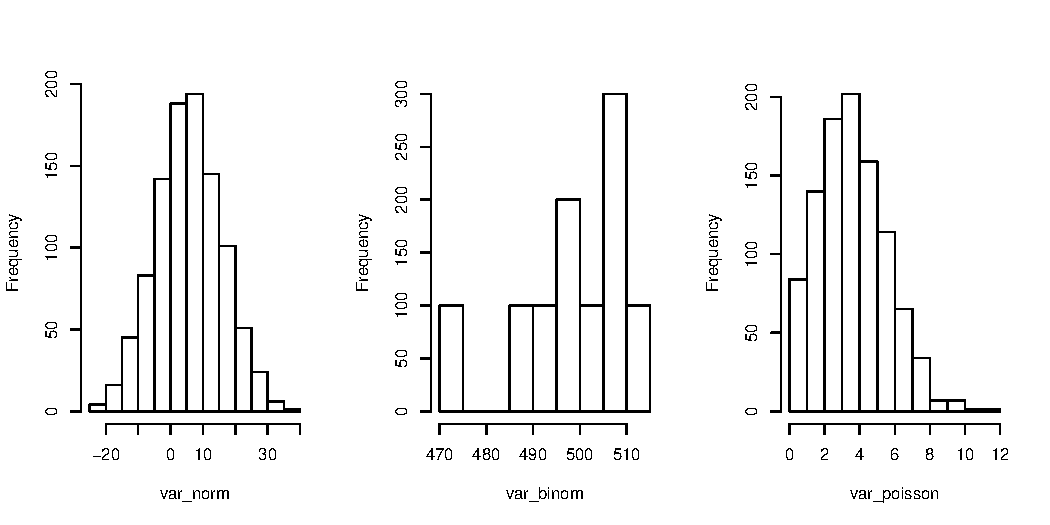
\includegraphics[width=\maxwidth]{figure/unnamed-chunk-2-1} 

\end{knitrout}

\section*{2. Subset data frame (4 points)}

\subsection*{a)}

Download the following data from \verb`WDI` and clean it as follows. Briefly comment on what each command does.

\begin{knitrout}
\definecolor{shadecolor}{rgb}{0.969, 0.969, 0.969}\color{fgcolor}\begin{kframe}
\begin{alltt}
\hlkwd{library}\hlstd{(WDI)}
\end{alltt}


{\ttfamily\noindent\itshape\color{messagecolor}{\#\# Loading required package: RJSONIO}}\begin{alltt}
\hlstd{d_wdi} \hlkwb{<-} \hlkwd{WDI}\hlstd{(}\hlkwc{indicator} \hlstd{=} \hlkwd{c}\hlstd{(}\hlstr{"NY.GDP.PCAP.CD"}\hlstd{,} \hlstr{"SP.DYN.IMRT.IN"}\hlstd{,} \hlstr{"SH.MED.PHYS.ZS"}\hlstd{),}
             \hlkwc{start} \hlstd{=} \hlnum{2005}\hlstd{,} \hlkwc{end} \hlstd{=} \hlnum{2010}\hlstd{,} \hlkwc{extra} \hlstd{=} \hlnum{TRUE}\hlstd{)}
\hlstd{d_wdi} \hlkwb{<-} \hlstd{d_wdi[d_wdi}\hlopt{$}\hlstd{region} \hlopt{!=} \hlstr{"Aggregates"}\hlstd{,}
       \hlkwd{c}\hlstd{(}\hlstr{"country"}\hlstd{,} \hlstr{"year"}\hlstd{,} \hlstr{"NY.GDP.PCAP.CD"}\hlstd{,} \hlstr{"SP.DYN.IMRT.IN"}\hlstd{,} \hlstr{"SH.MED.PHYS.ZS"}\hlstd{)]}
\hlkwd{colnames}\hlstd{(d_wdi)[}\hlnum{3}\hlopt{:}\hlnum{5}\hlstd{]} \hlkwb{<-} \hlkwd{c}\hlstd{(}\hlstr{'gdppc'}\hlstd{,} \hlstr{'infant_mortality'}\hlstd{,} \hlstr{'number_of_physician'}\hlstd{)}
\hlstd{d_wdi} \hlkwb{<-} \hlkwd{na.omit}\hlstd{(d_wdi)}
\end{alltt}
\end{kframe}
\end{knitrout}

\verb`infant_mortality`: number of mortality per 1000 live births

\verb`number_of_physician`: number of physician per 1000 people

\subsection*{b)}

Use subsetting techniques to do the following:

\begin{enumerate}
\item Show the GDP per capita of Brazil across years
\item Show the country-years where infant mortality $>$ 100 per 1000 live birth
\item Show the country-years where GDP per capita is above average
\item Show the country-years where GDP per capita is above average, but number of physician is below average
\end{enumerate}

\textbf{Solution}

\begin{knitrout}
\definecolor{shadecolor}{rgb}{0.969, 0.969, 0.969}\color{fgcolor}\begin{kframe}
\begin{alltt}
\hlkwd{library}\hlstd{(WDI)}

\hlcom{# Download data from WDI, specifying the indicators and start / end year}
\hlstd{d_wdi} \hlkwb{<-} \hlkwd{WDI}\hlstd{(}\hlkwc{indicator} \hlstd{=} \hlkwd{c}\hlstd{(}\hlstr{"NY.GDP.PCAP.CD"}\hlstd{,} \hlstr{"SP.DYN.IMRT.IN"}\hlstd{,} \hlstr{"SH.MED.PHYS.ZS"}\hlstd{),}
             \hlkwc{start} \hlstd{=} \hlnum{2008}\hlstd{,} \hlkwc{end} \hlstd{=} \hlnum{2010}\hlstd{,} \hlkwc{extra} \hlstd{=} \hlnum{TRUE}\hlstd{)}

\hlcom{# Remove aggregates rows, selecting wanted columns by name}
\hlstd{d_wdi} \hlkwb{<-} \hlstd{d_wdi[d_wdi}\hlopt{$}\hlstd{region} \hlopt{!=} \hlstr{"Aggregates"}\hlstd{,}
       \hlkwd{c}\hlstd{(}\hlstr{"country"}\hlstd{,} \hlstr{"year"}\hlstd{,} \hlstr{"NY.GDP.PCAP.CD"}\hlstd{,} \hlstr{"SP.DYN.IMRT.IN"}\hlstd{,} \hlstr{"SH.MED.PHYS.ZS"}\hlstd{)]}

\hlcom{# Rename some of the columns}
\hlkwd{colnames}\hlstd{(d_wdi)[}\hlnum{3}\hlopt{:}\hlnum{5}\hlstd{]} \hlkwb{<-} \hlkwd{c}\hlstd{(}\hlstr{'gdppc'}\hlstd{,} \hlstr{'infant_mortality'}\hlstd{,} \hlstr{'number_of_physician'}\hlstd{)}

\hlcom{# Remove all rows that have missing data}
\hlstd{d_wdi} \hlkwb{<-} \hlkwd{na.omit}\hlstd{(d_wdi)}
\end{alltt}
\end{kframe}
\end{knitrout}

\begin{knitrout}
\definecolor{shadecolor}{rgb}{0.969, 0.969, 0.969}\color{fgcolor}\begin{kframe}
\begin{alltt}
\hlcom{# 1. Show the GDP per capita of Brazil across years}
\hlstd{d_wdi[d_wdi}\hlopt{$}\hlstd{country} \hlopt{==} \hlstr{"Brazil"}\hlstd{,} \hlkwd{c}\hlstd{(}\hlstr{"country"}\hlstd{,} \hlstr{"year"}\hlstd{,} \hlstr{"gdppc"}\hlstd{)]}
\end{alltt}
\begin{verbatim}
##    country year     gdppc
## 94  Brazil 2008  8836.914
## 95  Brazil 2010 11318.057
\end{verbatim}
\begin{alltt}
\hlcom{# 2. Show the country-years where infant mortality > 100 per 1000 live birth}
\hlstd{d_wdi[d_wdi}\hlopt{$}\hlstd{infant_mortality} \hlopt{>} \hlnum{100}\hlstd{,} \hlkwd{c}\hlstd{(}\hlstr{"country"}\hlstd{,} \hlstr{"year"}\hlstd{,} \hlstr{"infant_mortality"}\hlstd{)]}
\end{alltt}
\begin{verbatim}
##                      country year infant_mortality
## 34                    Angola 2009            112.2
## 120 Central African Republic 2009            103.6
## 562             Sierra Leone 2010            107.0
## 563             Sierra Leone 2008            116.2
\end{verbatim}
\begin{alltt}
\hlcom{# 3. Show the country-years where GDP per capita is above average}
\hlstd{d_wdi[d_wdi}\hlopt{$}\hlstd{gdppc} \hlopt{>} \hlkwd{mean}\hlstd{(d_wdi}\hlopt{$}\hlstd{gdppc),} \hlkwd{c}\hlstd{(}\hlstr{"country"}\hlstd{,} \hlstr{"year"}\hlstd{,} \hlstr{"gdppc"}\hlstd{)]}
\end{alltt}
\begin{verbatim}
##                  country year     gdppc
## 16               Andorra 2010  42952.72
## 17               Andorra 2009  46401.09
## 20  United Arab Emirates 2010  33885.93
## 43               Austria 2010  46593.39
## 48             Australia 2010  51801.05
## 62              Barbados 2010  15854.36
## 67               Belgium 2010  44360.90
## 69               Belgium 2008  48561.36
## 76               Bahrain 2008  23037.64
## 77               Bahrain 2010  20545.75
## 88     Brunei Darussalam 2008  37094.86
## 89     Brunei Darussalam 2010  30882.40
## 99          Bahamas, The 2008  23674.14
## 113               Canada 2008  46400.44
## 114               Canada 2010  47463.63
## 124          Switzerland 2010  74277.12
## 154               Cyprus 2010  30438.90
## 155               Cyprus 2008  34950.35
## 157       Czech Republic 2008  22649.38
## 158       Czech Republic 2010  19763.96
## 160              Germany 2008  45632.84
## 162              Germany 2010  41725.85
## 167              Denmark 2009  57895.50
## 168              Denmark 2010  57647.67
## 182              Estonia 2008  18087.68
## 190                Spain 2010  30737.83
## 202              Finland 2009  47107.16
## 203              Finland 2010  46205.17
## 204              Finland 2008  53401.31
## 214               France 2008  45415.81
## 215               France 2010  40708.50
## 222       United Kingdom 2010  38362.22
## 245               Greece 2010  26863.01
## 246               Greece 2008  31700.49
## 267              Croatia 2008  15887.42
## 273              Hungary 2008  15598.32
## 278              Ireland 2008  60968.84
## 279              Ireland 2010  47903.68
## 280               Israel 2010  30551.12
## 295              Iceland 2008  55446.76
## 297              Iceland 2010  41695.89
## 298                Italy 2009  36995.11
## 299                Italy 2010  35877.87
## 300                Italy 2008  40659.67
## 310                Japan 2010  42909.23
## 312                Japan 2008  37865.62
## 334          Korea, Rep. 2008  20474.89
## 336          Korea, Rep. 2010  22151.21
## 337               Kuwait 2010  38580.41
## 338               Kuwait 2008  54540.42
## 339               Kuwait 2009  37158.42
## 367            Lithuania 2008  14961.72
## 371           Luxembourg 2010 102863.10
## 423                Malta 2010  19694.08
## 458          Netherlands 2010  50341.25
## 459          Netherlands 2008  56628.75
## 460               Norway 2009  80017.78
## 461               Norway 2010  87646.27
## 462               Norway 2008  96880.51
## 467          New Zealand 2010  33394.07
## 472                 Oman 2010  20922.66
## 474                 Oman 2008  23483.63
## 504             Portugal 2010  22539.99
## 512                Qatar 2010  71510.19
## 538         Saudi Arabia 2008  19714.40
## 539         Saudi Arabia 2010  19326.58
## 540         Saudi Arabia 2009  16013.28
## 550               Sweden 2008  55746.84
## 551               Sweden 2010  52076.43
## 552               Sweden 2009  46207.06
## 553            Singapore 2010  46569.69
## 556             Slovenia 2008  27501.82
## 558             Slovenia 2010  23417.64
## 560      Slovak Republic 2010  16509.90
## 626  Trinidad and Tobago 2010  15494.70
## 643        United States 2010  48374.06
## 644        United States 2009  47001.56
\end{verbatim}
\begin{alltt}
\hlcom{# 4. Show the country-years where GDP per capita is above average,}
\hlcom{# but number of physician is below average}
\hlstd{d_wdi[d_wdi}\hlopt{$}\hlstd{gdppc} \hlopt{>} \hlkwd{mean}\hlstd{(d_wdi}\hlopt{$}\hlstd{gdppc)} \hlopt{&}
        \hlstd{d_wdi}\hlopt{$}\hlstd{number_of_physician} \hlopt{<} \hlkwd{mean}\hlstd{(d_wdi}\hlopt{$}\hlstd{number_of_physician),}
      \hlkwd{c}\hlstd{(}\hlstr{"country"}\hlstd{,} \hlstr{"year"}\hlstd{,} \hlstr{"gdppc"}\hlstd{)]}
\end{alltt}
\begin{verbatim}
##                 country year    gdppc
## 76              Bahrain 2008 23037.64
## 77              Bahrain 2010 20545.75
## 88    Brunei Darussalam 2008 37094.86
## 89    Brunei Darussalam 2010 30882.40
## 538        Saudi Arabia 2008 19714.40
## 539        Saudi Arabia 2010 19326.58
## 540        Saudi Arabia 2009 16013.28
## 626 Trinidad and Tobago 2010 15494.70
\end{verbatim}
\end{kframe}
\end{knitrout}

\section*{3. Build linear model (4 points)}

\subsection*{a)}

Download 2 variables of interest and build a linear model of their relationship using \verb`lm()`. Show the \verb`summary()` of results

\subsection*{b)}

Show the result with \verb`stargazer`, customizing:
\begin{itemize}
\item The labels of the independent variables (i.e. the covariate)
\item The label of the dependent variable
\item Make the model name (i.e. OLS) show up
\end{itemize}

Hint: The options to do those things are in \verb`help(stargazer)`. I have worded the task in a way that should help you find the relevant options.

\textbf{Solution}

\begin{knitrout}
\definecolor{shadecolor}{rgb}{0.969, 0.969, 0.969}\color{fgcolor}\begin{kframe}
\begin{alltt}
\hlstd{m1} \hlkwb{<-} \hlkwd{lm}\hlstd{(infant_mortality} \hlopt{~} \hlstd{gdppc,} \hlkwc{data} \hlstd{= d_wdi)}
\hlkwd{summary}\hlstd{(m1)}
\end{alltt}
\begin{verbatim}
## 
## Call:
## lm(formula = infant_mortality ~ gdppc, data = d_wdi)
## 
## Residuals:
##     Min      1Q  Median      3Q     Max 
## -28.743 -17.413  -5.357  11.922  78.783 
## 
## Coefficients:
##               Estimate Std. Error t value Pr(>|t|)    
## (Intercept)  3.775e+01  1.713e+00   22.04   <2e-16 ***
## gdppc       -7.406e-04  6.908e-05  -10.72   <2e-16 ***
## ---
## Signif. codes:  0 '***' 0.001 '**' 0.01 '*' 0.05 '.' 0.1 ' ' 1
## 
## Residual standard error: 21.68 on 249 degrees of freedom
## Multiple R-squared:  0.3158,	Adjusted R-squared:  0.3131 
## F-statistic: 114.9 on 1 and 249 DF,  p-value: < 2.2e-16
\end{verbatim}
\end{kframe}
\end{knitrout}

\begin{kframe}
\begin{alltt}
\hlkwd{library}\hlstd{(stargazer)}
\end{alltt}


{\ttfamily\noindent\itshape\color{messagecolor}{\#\# \\\#\# Please cite as: \\\#\# \\\#\#\ \ Hlavac, Marek (2014). stargazer: LaTeX code and ASCII text for well-formatted regression and summary statistics tables.\\\#\#\ \ R package version 5.1. http://CRAN.R-project.org/package=stargazer}}\begin{alltt}
\hlkwd{stargazer}\hlstd{(m1,}
          \hlkwc{covariate.labels} \hlstd{=} \hlkwd{c}\hlstd{(}\hlstr{"GDP per capita"}\hlstd{),}
          \hlkwc{dep.var.labels} \hlstd{=} \hlkwd{c}\hlstd{(}\hlstr{"Infant Mortality (per 1000 births)"}\hlstd{),}
          \hlkwc{model.names} \hlstd{=} \hlnum{TRUE}\hlstd{)}
\end{alltt}
\end{kframe}
% Table created by stargazer v.5.1 by Marek Hlavac, Harvard University. E-mail: hlavac at fas.harvard.edu
% Date and time: Thu, Sep 17, 2015 - 11:55:39 AM
\begin{table}[!htbp] \centering 
  \caption{} 
  \label{} 
\begin{tabular}{@{\extracolsep{5pt}}lc} 
\\[-1.8ex]\hline 
\hline \\[-1.8ex] 
 & \multicolumn{1}{c}{\textit{Dependent variable:}} \\ 
\cline{2-2} 
\\[-1.8ex] & Infant Mortality (per 1000 births) \\ 
\\[-1.8ex] & \textit{OLS} \\ 
\hline \\[-1.8ex] 
 GDP per capita & $-$0.001$^{***}$ \\ 
  & (0.0001) \\ 
  & \\ 
 Constant & 37.753$^{***}$ \\ 
  & (1.713) \\ 
  & \\ 
\hline \\[-1.8ex] 
Observations & 251 \\ 
R$^{2}$ & 0.316 \\ 
Adjusted R$^{2}$ & 0.313 \\ 
Residual Std. Error & 21.678 (df = 249) \\ 
F Statistic & 114.948$^{***}$ (df = 1; 249) \\ 
\hline 
\hline \\[-1.8ex] 
\textit{Note:}  & \multicolumn{1}{r}{$^{*}$p$<$0.1; $^{**}$p$<$0.05; $^{***}$p$<$0.01} \\ 
\end{tabular} 
\end{table} 


\section*{4. Calculate sum of squares and RMSE (4 points)}

\begin{enumerate}
\item Extract the residuals and predicted values (fitted values) from the model object (from Question 3)
\item Calculate three ``sum of squares'' (TSS, RegSS, RSS)
\item Calculate the root mean square error and compare with R. (In R and stargazer, RMSE is called ``Residual standard error''.)
\end{enumerate}

Note: the data you feed to \verb`lm()` may have missing data, so R has to modify the data a little before using it. To extract the data that are actually used by \verb`lm()`, use \verb`my_model$model`. Use this data to calculate $\bar y$ in the sum of squares.

\textbf{Solution}

\begin{knitrout}
\definecolor{shadecolor}{rgb}{0.969, 0.969, 0.969}\color{fgcolor}\begin{kframe}
\begin{alltt}
\hlstd{res} \hlkwb{<-} \hlstd{m1}\hlopt{$}\hlstd{residuals} \hlcom{# Residuals}
\hlstd{pred} \hlkwb{<-} \hlstd{m1}\hlopt{$}\hlstd{fitted.values} \hlcom{# Predicted values}
\hlstd{y} \hlkwb{<-} \hlstd{m1}\hlopt{$}\hlstd{model}\hlopt{$}\hlstd{infant_mortality} \hlcom{# Data of Y that is used by lm()}

\hlcom{# Calculate 3 sum of squares}
\hlstd{TSS} \hlkwb{<-} \hlkwd{sum}\hlstd{( (y} \hlopt{-} \hlkwd{mean}\hlstd{(y))} \hlopt{**} \hlnum{2}\hlstd{)}
\hlstd{RegSS} \hlkwb{<-} \hlkwd{sum}\hlstd{( (pred} \hlopt{-} \hlkwd{mean}\hlstd{(y))} \hlopt{**} \hlnum{2}\hlstd{)}
\hlstd{RSS} \hlkwb{<-} \hlkwd{sum}\hlstd{( res} \hlopt{**} \hlnum{2} \hlstd{)}

\hlcom{# Calculate root mean square error}
\hlstd{N} \hlkwb{<-} \hlkwd{nrow}\hlstd{(d_wdi)}
\hlstd{k} \hlkwb{<-} \hlnum{1} \hlcom{# We only have 1 predictor, which is log_gdppc}
\hlstd{rmse} \hlkwb{<-} \hlkwd{sqrt}\hlstd{(RSS} \hlopt{/} \hlstd{(N} \hlopt{-} \hlstd{k} \hlopt{-} \hlnum{1}\hlstd{))}
\end{alltt}
\end{kframe}
\end{knitrout}

The calculated root mean square error is 21.6783991, the same as reported by R in \verb`summary(m1)`.


\end{document}
